\documentclass[12pt,a4paper]{article}
\input{../mltshorts.de/mlt_shorts}
\begin{document}

\capbsp{Visualisierung Dopplerefekt}

Der Dopplereffekt ist jener Effekt, der die Frequenz eines Tons, welcher von
einer Schallquelle ausgeht, scheinbar ver�ndert, wenn sich der Beobachter
relativ zur Schallquelle bewegt. Sie sollen nun ein \matlab-Script
\begin{verbatim}
schall
\end{verbatim}
schreiben, welches mithilfe der Funktion \verb�kreisf1� diesen Effekt 
visualisiert. Daf�r m�ssen Sie zuerst die Aufgaben {\bf Kreisparametrisierung}
und {\bf Errormeldung Kreis} abgeben, weil \verb�kreisf1� dort erstellt wird.

Die Visualisierung soll durch eine Momentaufnahme der bewegten Schallquelle und
den davor ausgesandten Wellenfronten geschehen (siehe Grafik).\\
Die Vorgaben sind folgende: Die Schallquelle bewegt sich vom Koordinatenursprung
von Links nach Rechts, mit einer bestimmten Geschwindigkeit $v$. Die
Momentaufnahme wird nach genau einer Sekunde gemacht. Darin sollen 50
Wellenfronten dieser ersten Sekunde der Bewegung erkennbar sein, sowie die
Positionen der Schallquelle, an denen die betrachteten Wellenfronten ausgesandt
wurden (gleichm��ige Abst�nde). Die
Schallgeschwindigkeit betr�gt 337,5 m/s (bei angenommenen 10�C). Speichern Sie
diesen Wert als Variable $c$.\\\\
Programmieren Sie das Skript zuerst nur f�r
eine Geschwindigkeit 
$v=c/2$. Zeichnen Sie die Kreise mit \verb�kreisf1� mit jeweils \verb�n = 50�
Punkten. Verwenden
Sie auf jeden Fall zur besseren Darstellung \matref{axis equal}{axis}
und \matref{axis off}{axis}. Dann sollte Ihr Bild in etwa so aussehen:
\begin{center}
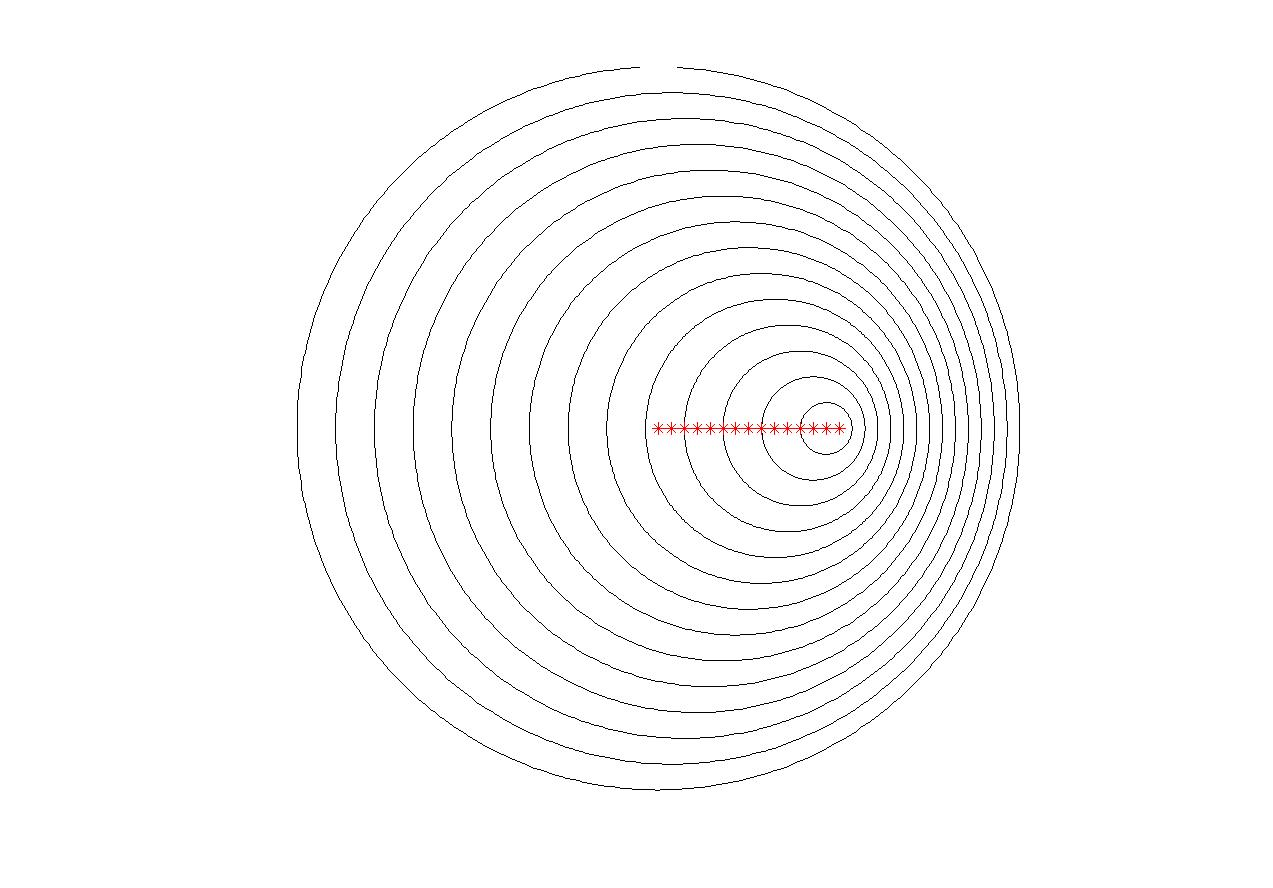
\includegraphics[width=0.7\textwidth]{doppler.jpg}
\end{center}
Danach erweitern Sie Ihr Skript, sodass drei \matref{figures}{figure} nacheinander
erstellt
weden. Die Geschwindigkeiten der Schallquelle sollen dabei folgende Werte
annehmen:
\begin{center}
\begin{tabular}{c|l}
  {\sc figure-Nummer} & {\sc v=}\\
  \hline \hline
  $1$ & $c/2$\\
  $2$ & $c$\\
  $3$ & $2\cdot c$\\       
\end{tabular}
\end{center}
Die Mittelpunkte sollen als rote * eingezeichnet werden. Betiteln Sie den \matrefe{plot}
im jeweiligen \matrefe{figure} mit dem verwendeten Geschwindigkeitswert 
($v=\ldots$).\\
\hline
\textbf{Wichtig:} Die Beziehung zwischen \matref{figures}{figure} und den
Geschwindigkeiten muss genau so wie in der obigen Tabelle sein. Weiters
m�ssen - um den automatischen test zu bestehen -  in der \matrefe{figure} zuerst
einzeln die Kreise (beginnend mit dem gr��ten), und nach allen Kreisen die
Mittelpunkte gezeichnet werden. Zeichnen Sie die Mittelpunkte mit
nur einem Befehl und ohne Schleife (Vektor mit den Koordinaten Mx bzw. My).\\\\
\hw Die Gleichung, mit der Sie zu den x-Werten der Mittelpunktskoordinaten
kommen, ist:
\begin{equation}
Mx=v\cdot t
\end{equation}
Verwenden Sie zur Berechnung von \verb�My� den Befehl \matrefe{zeros}.\\\\
\hw Bedenken Sie, dass die Kreise vom gr��ten zum kleinsten gezeichnet werden
sollen. Die Werte im Zeitvektor \verb�t� sind allerdings aufsteigend
(\verb�t(1)� ist der kleinste Wert, \verb�t(50)� der gr��te). Verwenden Sie also
die Gleichung
\begin{equation}
r=c\cdot t
\end{equation}
zur Berechnung der Radien, so sind auch die Werte im Vektor \verb�r�
aufsteigend. Sie m�ssen also den erhaltenen Vektor noch ``umdrehen'', damit die
Werte - wie verlangt - absteigend im Vektor stehen. Daf�r eignet sich  der
Befehl \matrefe{fliplr} sehr gut. 
\end{document}